\documentclass[aspectratio=169,usenames,dvipsnames]{beamer}

\usetheme{default}  % You can choose any other theme you prefer

\title{02 - Algoritmos}
\author{Mateus Oliveira de Figueiredo}
\date{29 de agosto de 2023}

\usepackage{tikz}
\usepackage{multicol}
\usepackage{algorithm}
\usepackage{algpseudocode}
\usepackage{xcolor}
\usepackage[portuguese]{babel}

\begin{document}

\begin{frame}
\titlepage
\end{frame}

\begin{frame}
\frametitle{Triangulação}
  \begin{block}{Problema}
    Dado um polígono, listar triângulos de alguma triangulação.
  \end{block}
  % 2 colunas
  \begin{columns}
    \column{0.5\textwidth}
    \begin{center}
      \begin{figure}
        \onslide<2->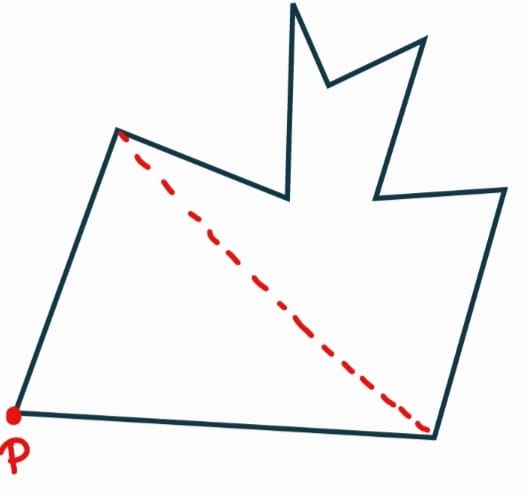
\includegraphics[width=0.95\textwidth]{figures/exemplo_0.jpeg}
      \end{figure}
    \end{center}
    \column{0.5\textwidth}
    \begin{center}
      \begin{figure}
        \onslide<3>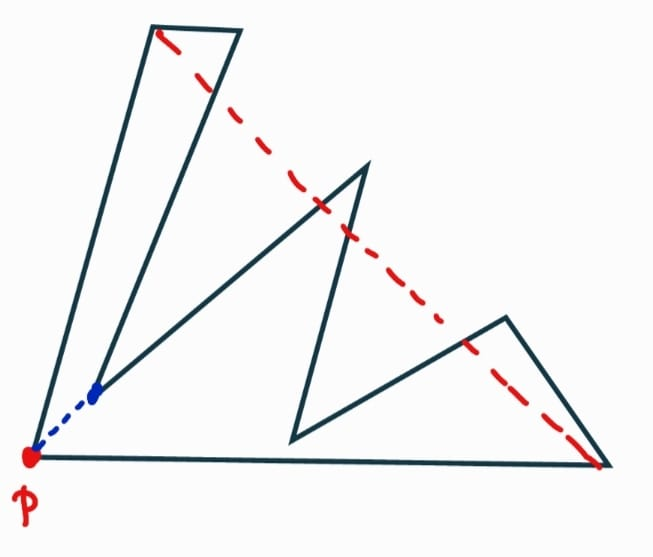
\includegraphics[width=0.95\textwidth]{figures/exemplo_1.jpeg}
      \end{figure}
    \end{center}
  \end{columns}
\end{frame}

\begin{frame}
\frametitle{Exemplos Utilizados}
  % add two columns to the slide
  \begin{columns}
    \column{0.32\textwidth}
    \begin{center}
        \begin{figure}
          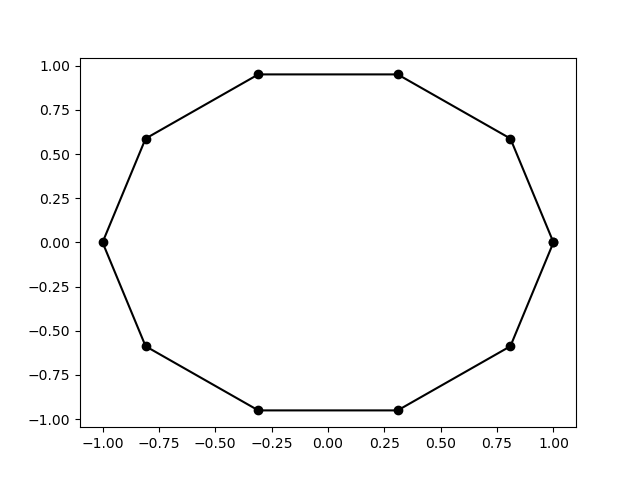
\includegraphics[width=0.95\textwidth]{figures/regular_10.png}
          \caption{Polígono Regular}
        \end{figure}
    \end{center}
    \column{0.32\textwidth}
    \begin{center}
        \begin{figure}
          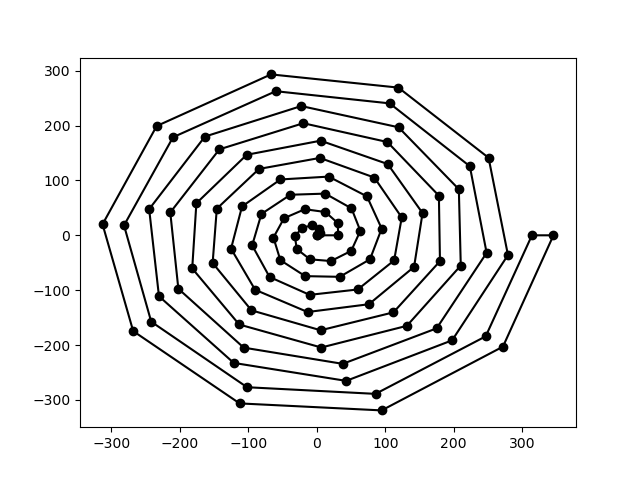
\includegraphics[width=0.95\textwidth]{figures/spiral_100.png}
        \caption{Espiral}
        \end{figure}
    \end{center}
    \column{0.32\textwidth}
    \begin{center}
        \begin{figure}
          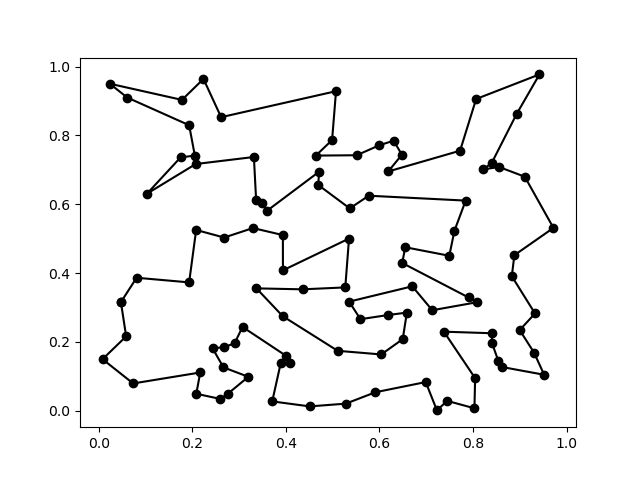
\includegraphics[width=0.95\textwidth]{figures/polygon_100_1.png}
          \caption{Caixeiro Viajante}
        \end{figure}
    \end{center}
  \end{columns}
\end{frame}


\begin{frame}{Resultados triangulação}
  \begin{columns}
    \column{0.5\textwidth}
    \begin{center}
      \begin{figure}
        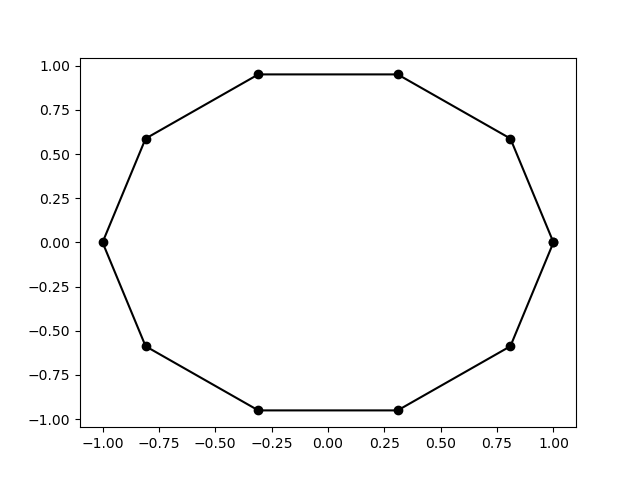
\includegraphics[width=0.95\textwidth]{figures/regular_10.png}
      \end{figure}
    \end{center}
    \column{0.5\textwidth}
    \begin{center}
      \begin{figure}
        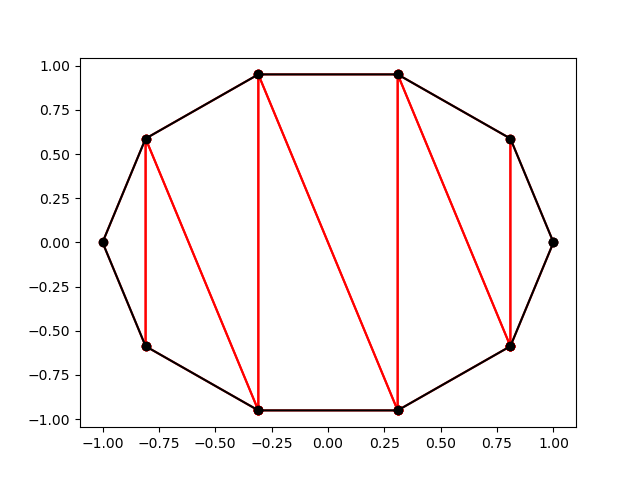
\includegraphics[width=0.95\textwidth]{figures/regular_10_trig.png}
      \end{figure}
    \end{center}
  \end{columns}
\end{frame}

\begin{frame}{Resultados triangulação}
  \begin{columns}
    \column{0.5\textwidth}
    \begin{center}
      \begin{figure}
        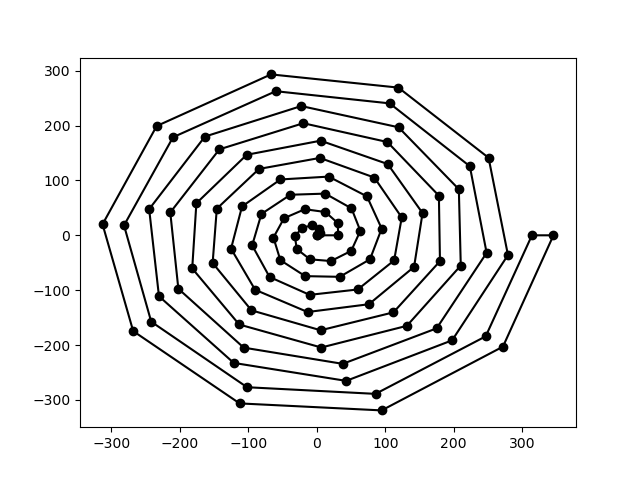
\includegraphics[width=0.95\textwidth]{figures/spiral_100.png}
      \end{figure}
    \end{center}
    \column{0.5\textwidth}
    \begin{center}
      \begin{figure}
        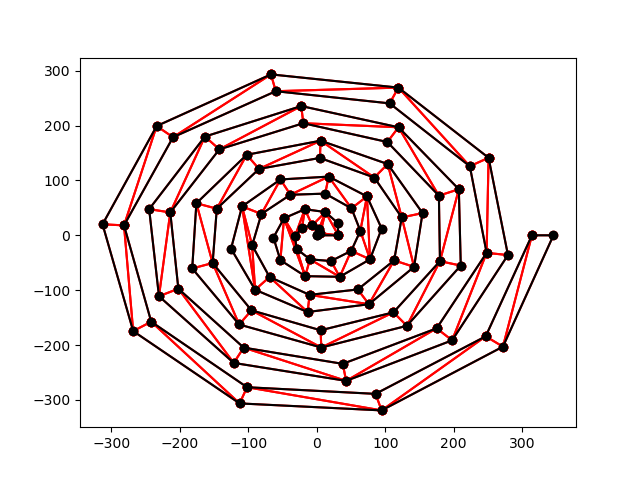
\includegraphics[width=0.95\textwidth]{figures/spiral_100_trig.png}
      \end{figure}
    \end{center}
  \end{columns}
\end{frame}

\begin{frame}{Resultados triangulação}
  \begin{columns}
    \column{0.5\textwidth}
    \begin{center}
      \begin{figure}
        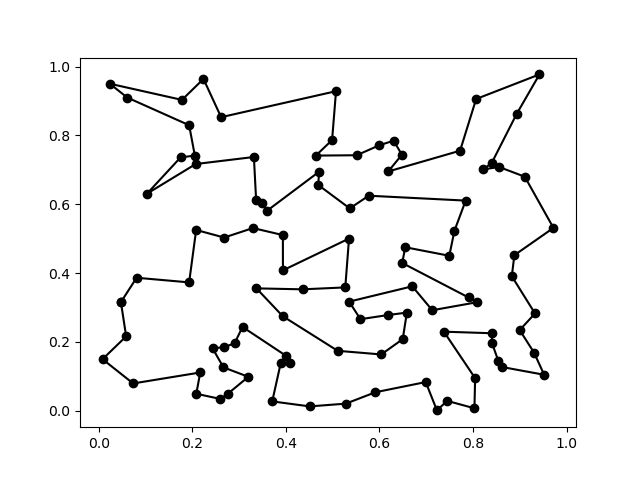
\includegraphics[width=0.95\textwidth]{figures/polygon_100_1.png}
      \end{figure}
    \end{center}
    \column{0.5\textwidth}
    \begin{center}
      \begin{figure}
        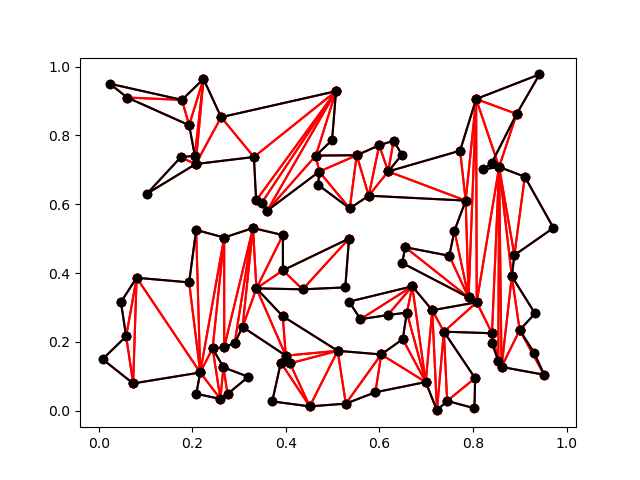
\includegraphics[width=0.95\textwidth]{figures/polygon_100_1_trig.png}
      \end{figure}
    \end{center}
  \end{columns}
\end{frame}

\begin{frame}{Resultados triangulação - Polígono não-simples}
    \begin{center}
      \begin{figure}
        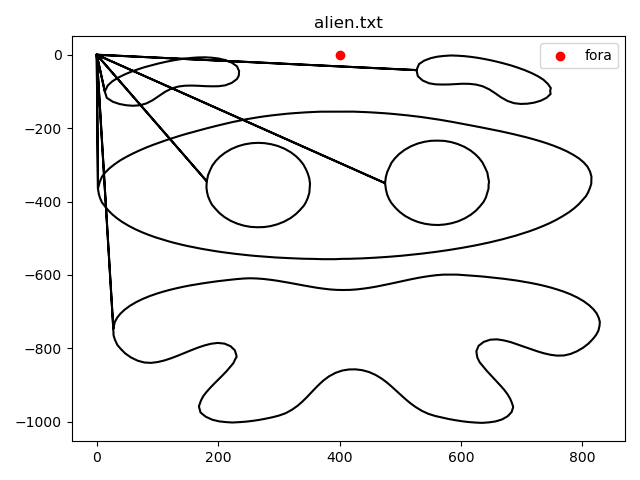
\includegraphics[width=0.7\textwidth]{figures/alien.png}
      \end{figure}
    \end{center}
\end{frame}

\begin{frame}{Performance}
  % 2 add two columns
  \begin{figure}
    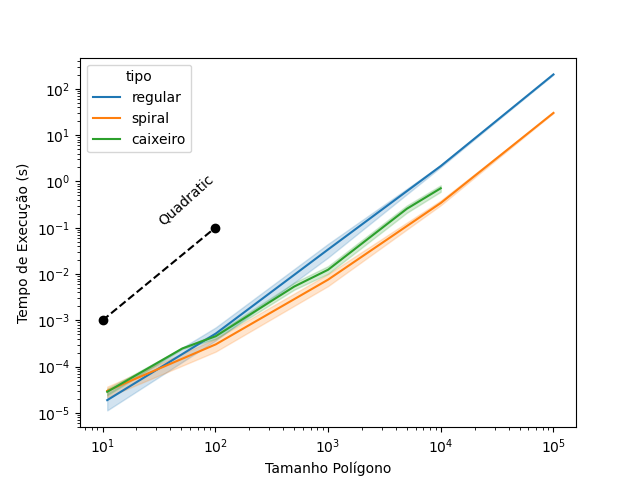
\includegraphics[width=0.7\textwidth]{figures/performance.png}
  \end{figure}
  \begin{center}
  Linha pontilhada representa uma função quadrática.
  \end{center}
\end{frame}

\begin{frame}
  \frametitle{Câmeras na Galeria de Arte}
  \begin{columns}
    \column{0.5\textwidth}
    \begin{center}
      \begin{itemize}
        \item Posicionar câmeras em uma galeria de arte de forma a cobrir toda a região interior.
      \end{itemize}
    \end{center}
    \column{0.5\textwidth}
    \begin{center}
      \begin{figure}
        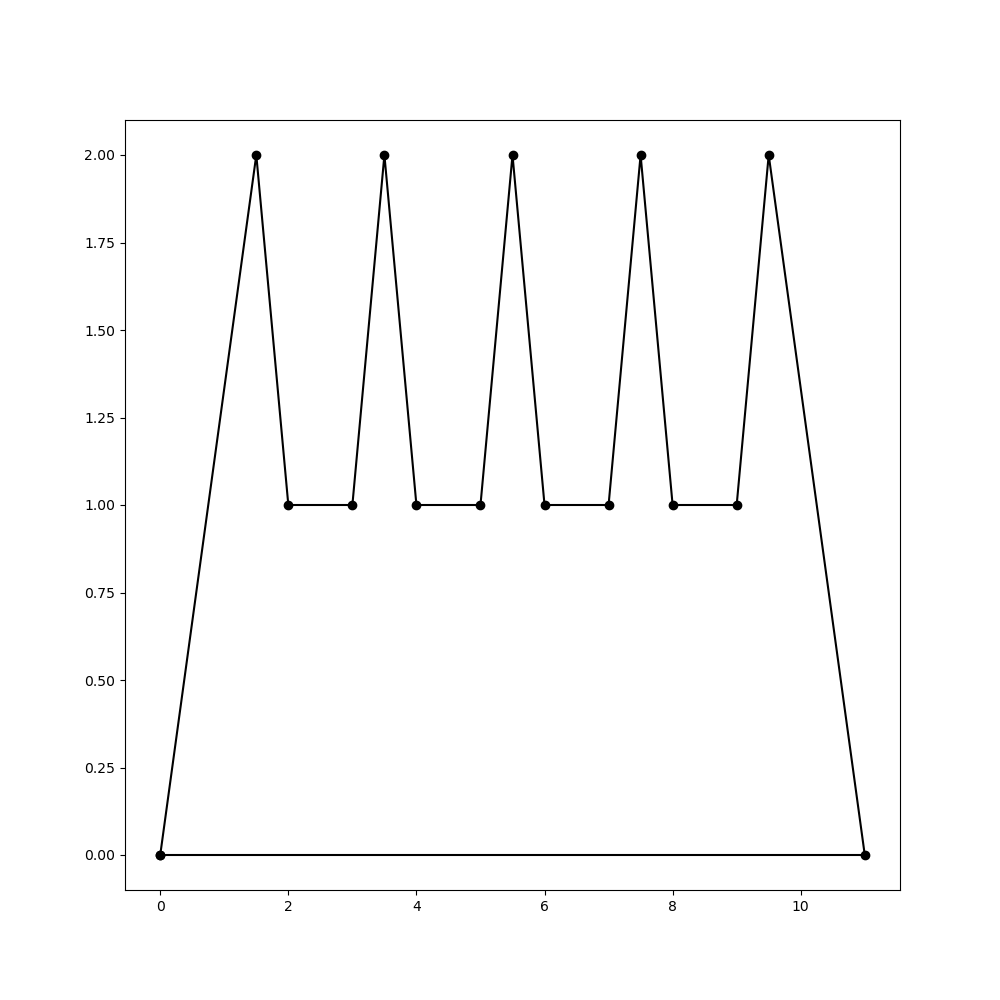
\includegraphics[width=0.95\textwidth]{figures/conr_example.png}
      \end{figure}
    \end{center}
  \end{columns}
\end{frame}

\begin{frame}{Algoritmo de Coloração}
  % Adicionar duas columnas
  \begin{columns}
    \column{0.5\textwidth}
    \begin{center}
      \begin{itemize}
        \item Kooshesh–Moret (1992), Three-coloring the vertices of a triangulated simple polygon
      \end{itemize}
    \end{center}
    \column{0.5\textwidth}
    \begin{center}
      \begin{figure}
        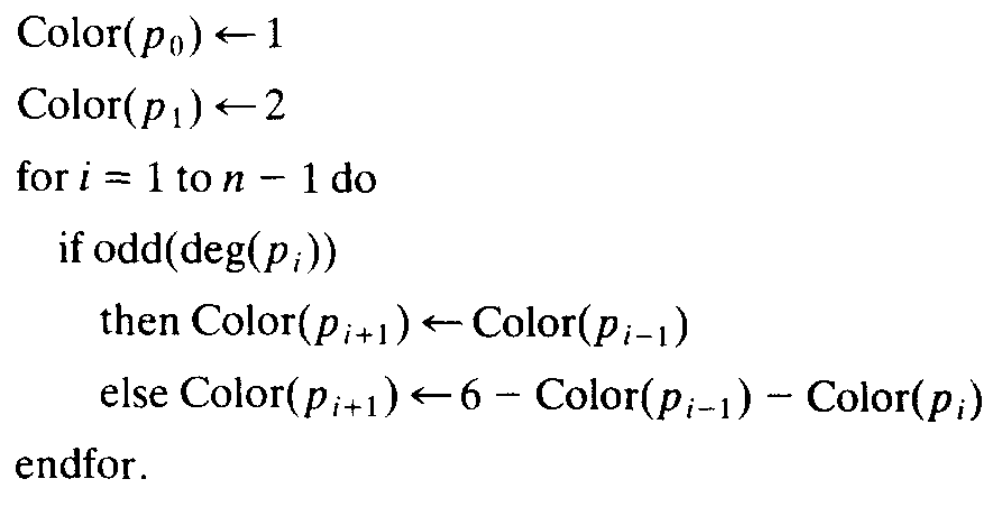
\includegraphics[width=0.95\textwidth]{figures/coloracao.png}
      \end{figure}
    \end{center}
  \end{columns}
\end{frame}

\begin{frame}{Algoritmo de Coloração}
  % Adicionar duas columnas
   % Adicionar duas columnas
    \begin{columns}
      \column{0.5\textwidth}
      \begin{center}
        \begin{figure}
        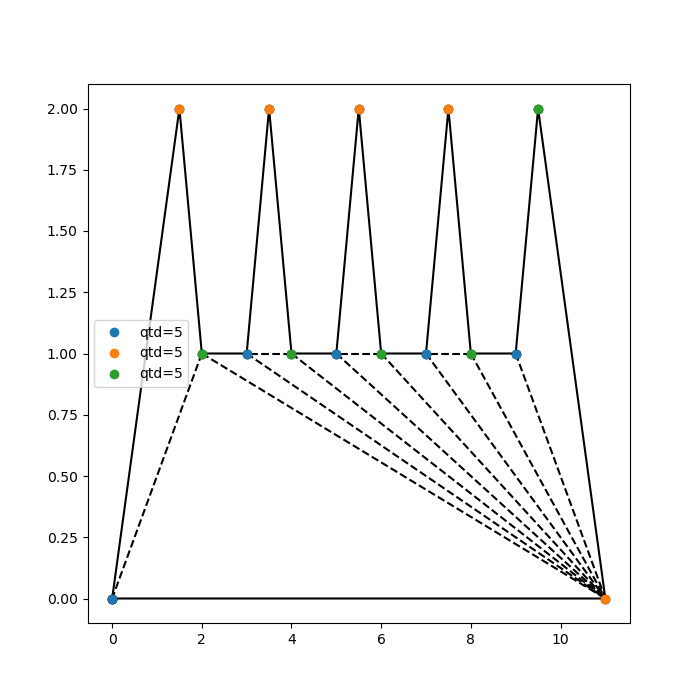
\includegraphics[width=0.95\textwidth]{figures/corn_example_coloring.png}
        \end{figure}
      \end{center}
      \column{0.5\textwidth}
    \begin{center}
      \begin{figure}
        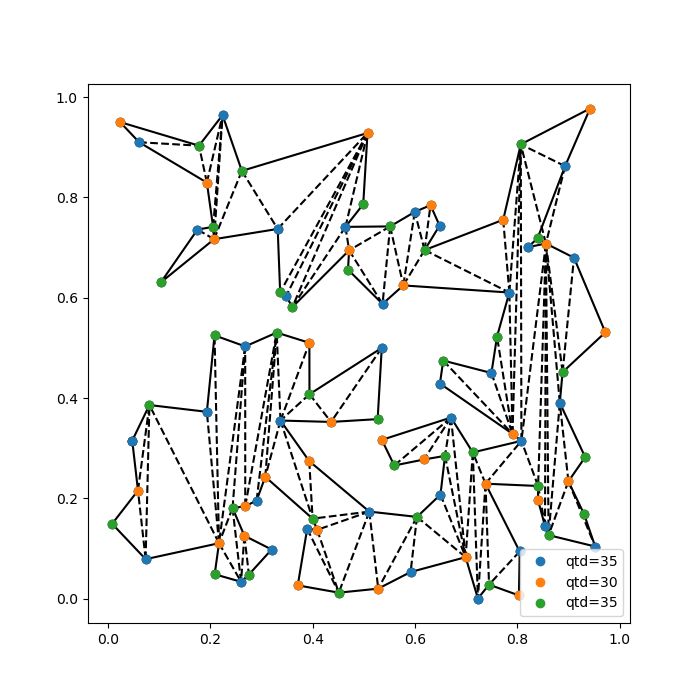
\includegraphics[width=0.95\textwidth]{figures/caxeiro_color.png}
      \end{figure}
    \end{center}
  \end{columns}
\end{frame}

% Adicionar slide com Obrigado
\begin{frame}
  \frametitle{}
  \begin{center}
    \Huge{Obrigado!}
  \end{center}
\end{frame}


\end{document}
